\documentclass[
	aspectratio=169, 
	8pt 
]{beamer}
\usepackage[utf8]{inputenc} 
\usepackage[ngerman]{babel}

\usepackage{fancybeamer} 
\usepackage{../vendor/fancyqr/fancyqr}

\usepackage{listings}
\usepackage{graphicx}
\usepackage{tikz}


%%%%%%%%%%%%%%%%%%%%%%%%%%%%%%%%%%%%%%%%%%%%%%%%%%%%%%%%%%%%%%%%%%%%%%
%\annotatedFigureBoxCustom{bottom-left}{top-right}{label}{label-position}{box-color}{label-color}{border-color}{text-color}
\newcommand*\annotatedFigureBoxCustom[8]{\draw[#5,thick,rounded corners] (#1) rectangle (#2);\node at (#4) [fill=#6,thick,shape=circle,draw=#7,inner sep=2pt,font=\sffamily,text=#8] {\textbf{#3}};}
%\annotatedFigureBox{bottom-left}{top-right}{label}{label-position}
\newcommand*\annotatedFigureBox[4]{\annotatedFigureBoxCustom{#1}{#2}{#3}{#4}{black}{white}{black}{black}}
\newcommand*\annotatedFigureText[4]{\node[draw=none, anchor=south west, text=#2, inner sep=0, text width=#3\linewidth,font=\sffamily] at (#1){#4};}
\newenvironment {annotatedFigure}[1]{\centering\begin{tikzpicture}
    \node[anchor=south west,inner sep=0] (image) at (0,0) { #1};\begin{scope}[x={(image.south east)},y={(image.north west)}]}{\end{scope}\end{tikzpicture}}
%%%%%%%%%%%%%%%%%%%%%%%%%%%%%%%%%%%%%%%%%%%%%%%%%%%%%%%%%%%%%%%%%%%%%%


\title{How-To-Studium} % short title is used for the slide footer but optional
%\subtitle{Epic Gamer Guide To Studium} % subtitles are optional at all
\author{Lars Pfrenger} % short author title is used for the slide footer but optional
\date{07. Oktober 2024} 

\begin{document}

\maketitle[assets/uni.png][50] % title slide with optional title picture and parameter to move it upwards

\section{Willkommen}

\section{Übersicht}

\subsection{Studienplan}
\begin{frame}{\insertsubsection}
    \begin{fancycolumns}[widths={48}]
        \fancyqr[height=0.8\linewidth]{https://www.uni-ulm.de/in/fakultaet/studium/plaene-ordnungen/pruefungsordnungen/}
        \nextcolumn
        \includegraphics[height=0.7\pdfpageheight, trim={1cm 11cm 1cm 2.2cm}, clip]{assets/SP-BA-Inf-FSPO2022.pdf}
    \end{fancycolumns}
\end{frame}

\begin{frame}{\insertsubsection}
    \includegraphics[width=\linewidth, trim={1cm 20.1cm 1cm 2.2cm}, clip]{assets/SP-BA-Inf-FSPO2022.pdf}
\end{frame}

\subsection{LP und SWS}
\begin{frame}{\insertsubsection}
    \begin{fancycolumns}[T]

        \begin{definition}{Leistungspunkte (LP / ECTS)\footnotemark[1]}
            \begin{itemize}
                \item Vergabe bei erfolgreichem Abschluss eines Moduls (Prüfung bestanden)
                \item Insgesamt $180$ LP für den Bachelor
                \item $\approx 30$ pro Semester
                \item $1 \text{ LP } \hat{=} \text{ } 30$ Stunden pro Semester
            \end{itemize}
        \end{definition}

        \nextcolumn
        
        \begin{definition}{Semesterwochenstunden (SWS)\footnotemark[2]}
            \begin{itemize}
                \item Anzahl der Stunden, welche ein Modul pro Woche einnimmt
                \item 1 SWS $\hat{=}$ $45$ min
                \item Unterteilt in Vorlesung, Übung und Projekt
            \end{itemize}
        \end{definition}
    \end{fancycolumns}

    \footnotetext[1]{\url{https://www.student.uni-stuttgart.de/uni-a-bis-z/ECTS-Credits-Leistungspunkte/}}
    \footnotetext[2]{\url{https://www.student.uni-stuttgart.de/uni-a-bis-z/SWS--Semesterwochenstunde/}}
\end{frame}


\subsection{Regelstudienzeit}
\begin{frame}{\insertsubsection}
    \begin{itemize}
        \item Plan ist nur eine Empfehlung. Man kann Module vorziehen oder nach hinten schieben.
        \item \textbf{Aber}: Orientierungsprüfungen beachten! 
        \item Max. 10 Semester
    \end{itemize}
\end{frame}
    
\subsection{Stundenplan}
\begin{frame}{\insertsubsection}
    \begin{fancycolumns}[widths={30}]
        \fancyqr[height=\linewidth]{https://www.uni-ulm.de/fileadmin/website_uni_ulm/iui2/dokumente/Stundenplaene/Stundenplaene-2024-SoSe/2024-WiSe-Stundenplaene_FSPO2022.pdf}
        \nextcolumn
        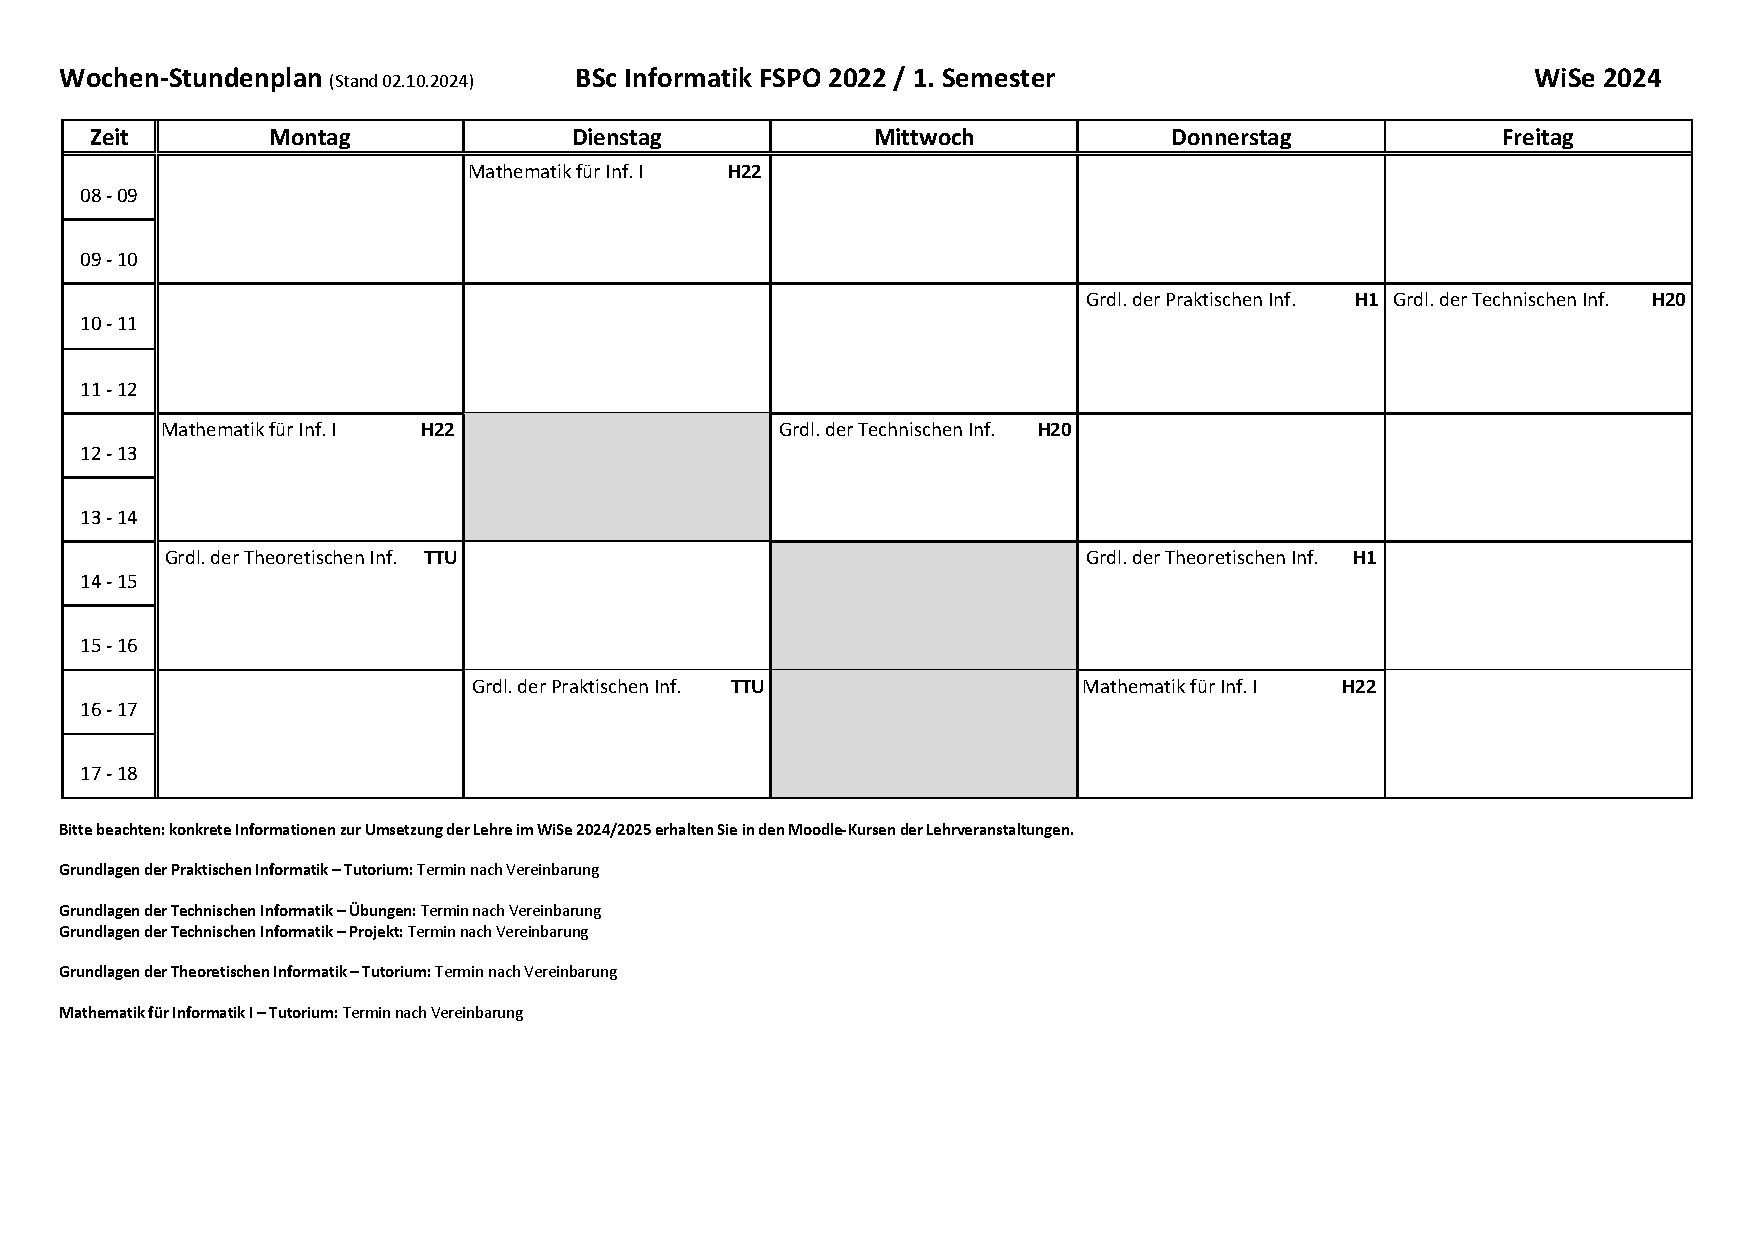
\includegraphics[width=\linewidth, trim={1cm 7.4cm 1cm 2cm}, clip, page=1]{assets/2024-WiSe-Stundenplaene_FSPO2022.pdf}
    \end{fancycolumns} 
\end{frame}


\subsection{Wo bekommt man mehr Infos?}
\begin{frame}{\insertsubsection}
    \begin{itemize}
        \item Campusonline / LSF
        \item Moodle
        \item E-Mail
        \item Portal / kiz Web-Services
    \end{itemize}
\end{frame}

\subsection{LSF}
\begin{frame}{\insertsubsection \space|\space\underline{\href{https://campusonline.uni-ulm.de}{campusonline.uni-ulm.de}}}
    \begin{itemize}
        \item Prüfungsanmeldung
        \item Transcript of Records
        \item Veranstaltungsverzeichnis
        \item Offizielle Verwaltung!
    \end{itemize}
\end{frame}

\begin{frame}{\insertsubsection \space|\space\underline{\href{https://campusonline.uni-ulm.de}{campusonline.uni-ulm.de}}}
    \begin{annotatedFigure}
        {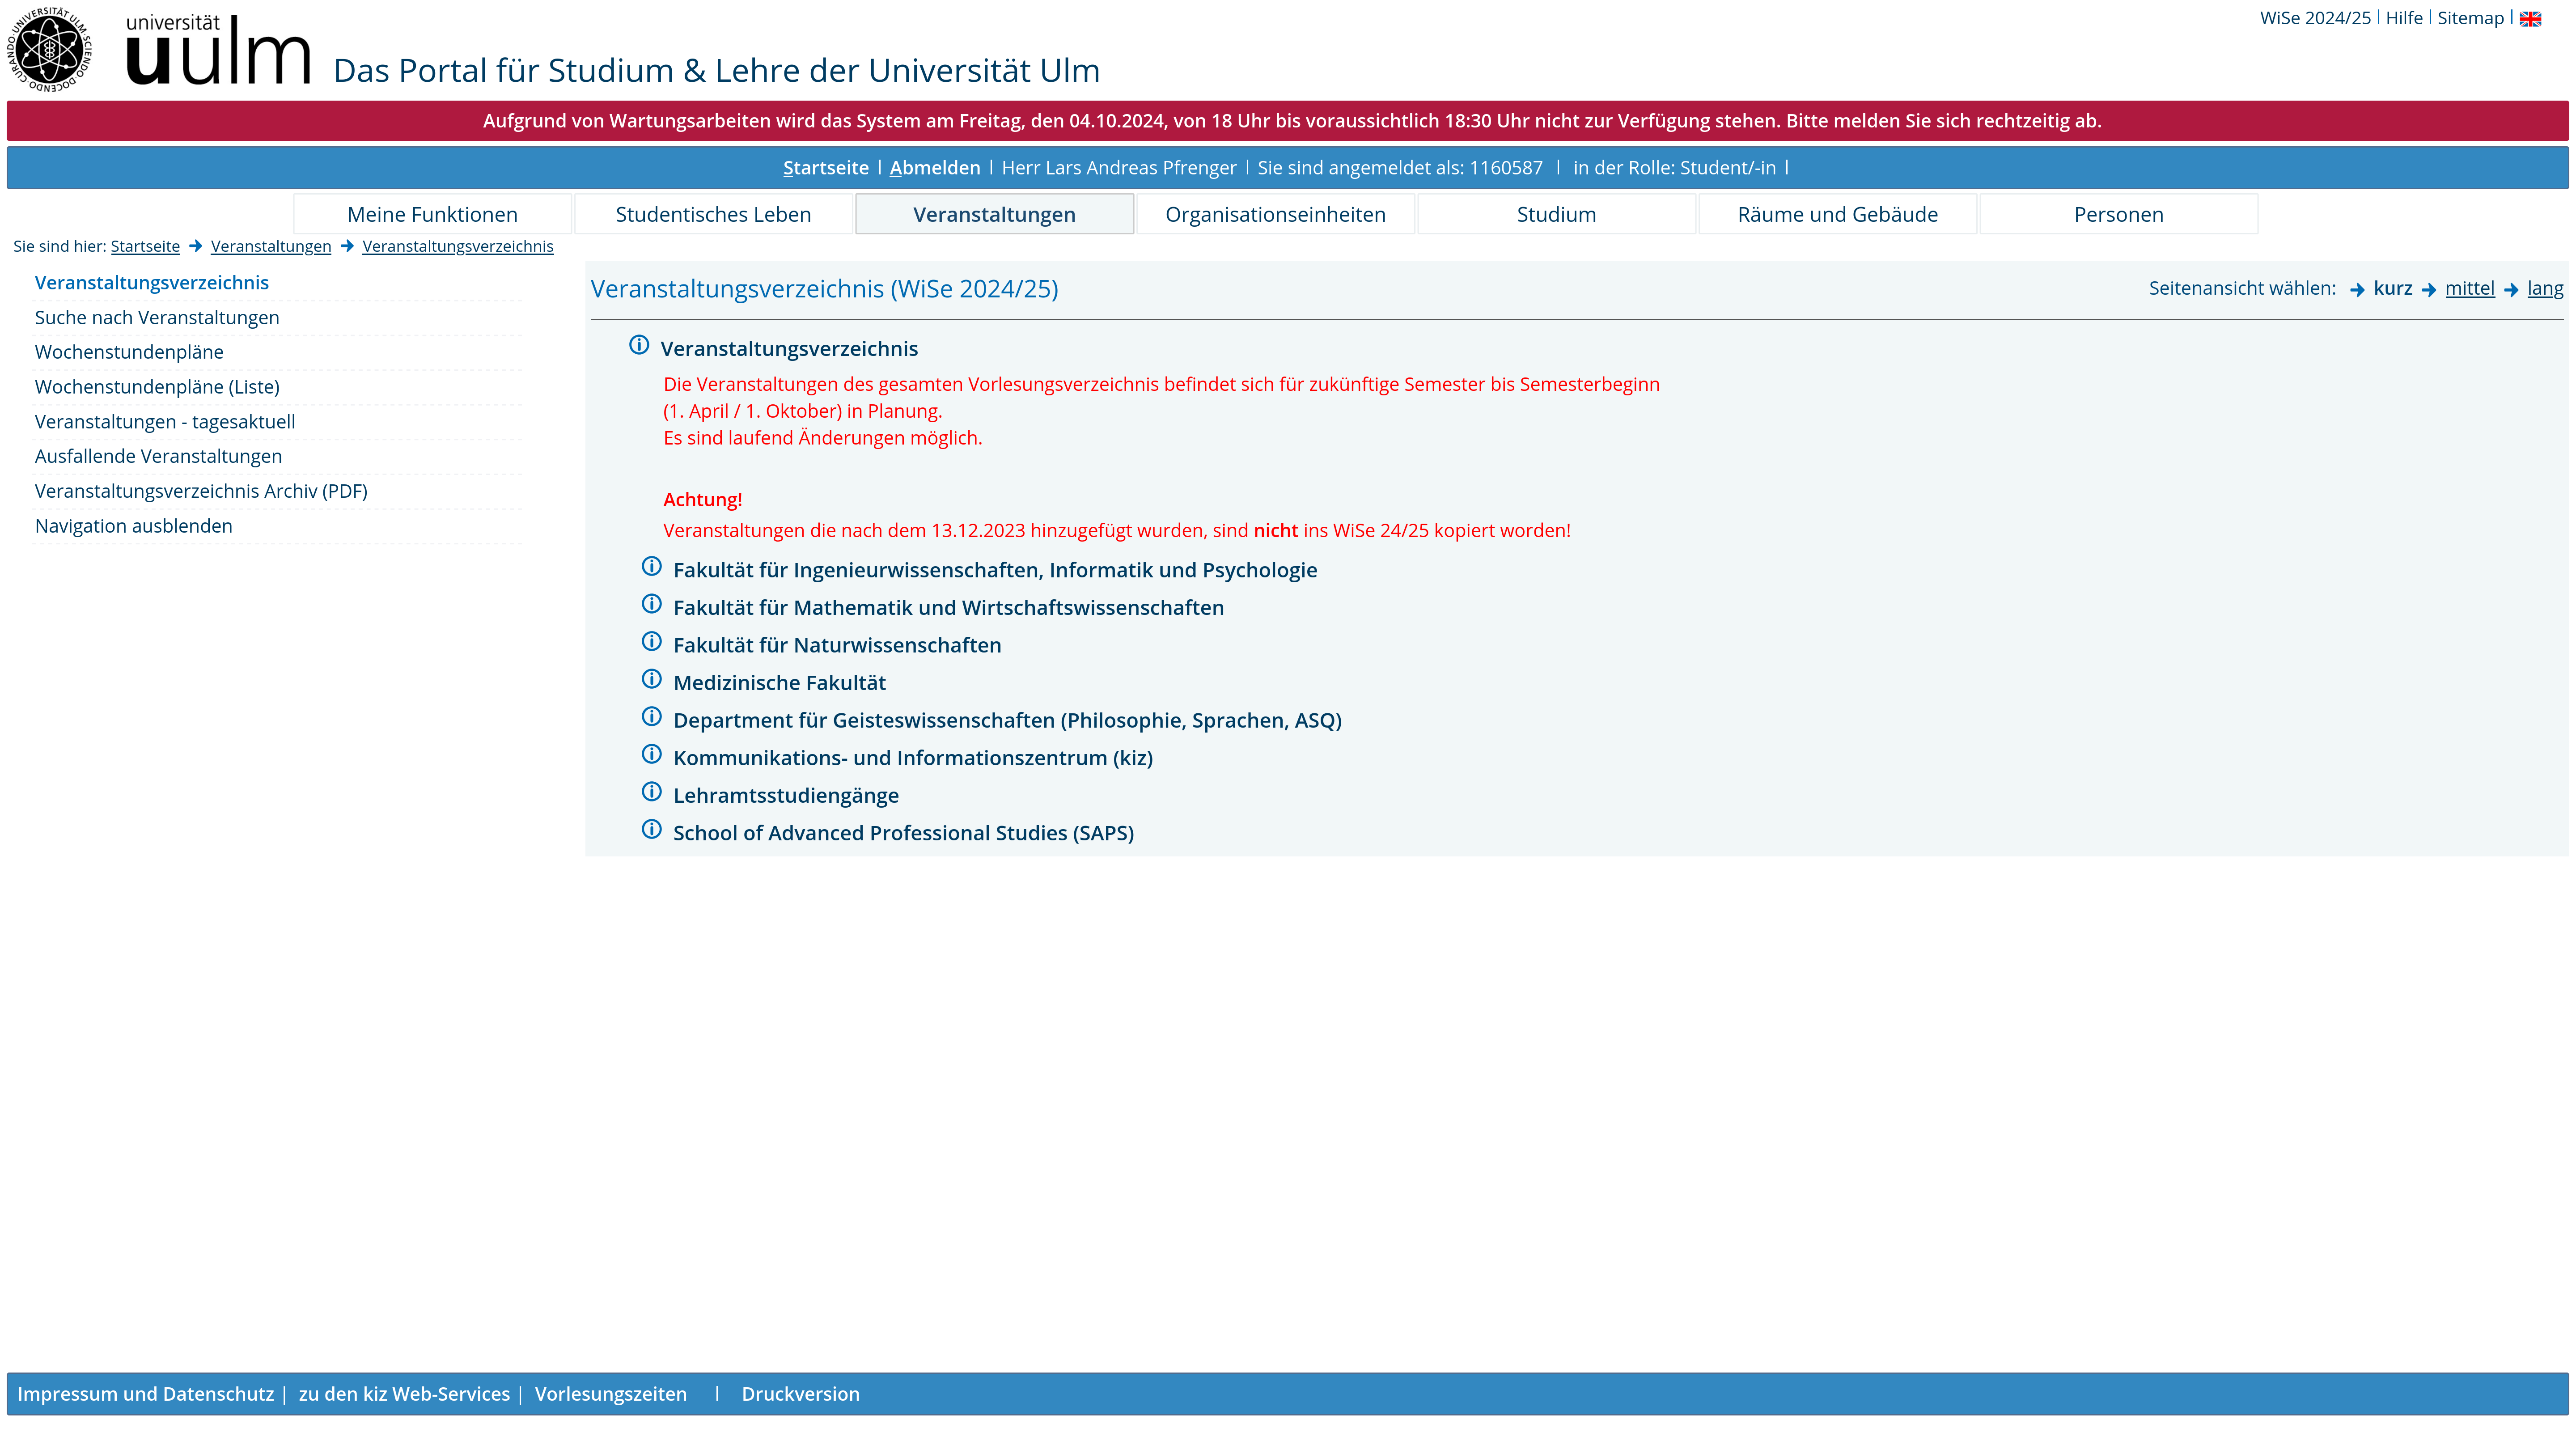
\includegraphics[clip, trim={0 0 0 0}, width=\linewidth]{assets/lsf-1.png}}
        \annotatedFigureBox{0.3328,0.8382}{0.444,0.8654}{A}{0.3328,0.8382}%bl
        \annotatedFigureBox{-0.001,0.7902}{0.111,0.8225}{B}{-0.001,0.7902}%bl
        \annotatedFigureBox{0.231,0.5911}{0.523,0.6268}{C}{0.231,0.5911}%bl
    \end{annotatedFigure}
\end{frame}


\begin{frame}{\insertsubsection \space|\space\underline{\href{https://campusonline.uni-ulm.de}{campusonline.uni-ulm.de}}}
    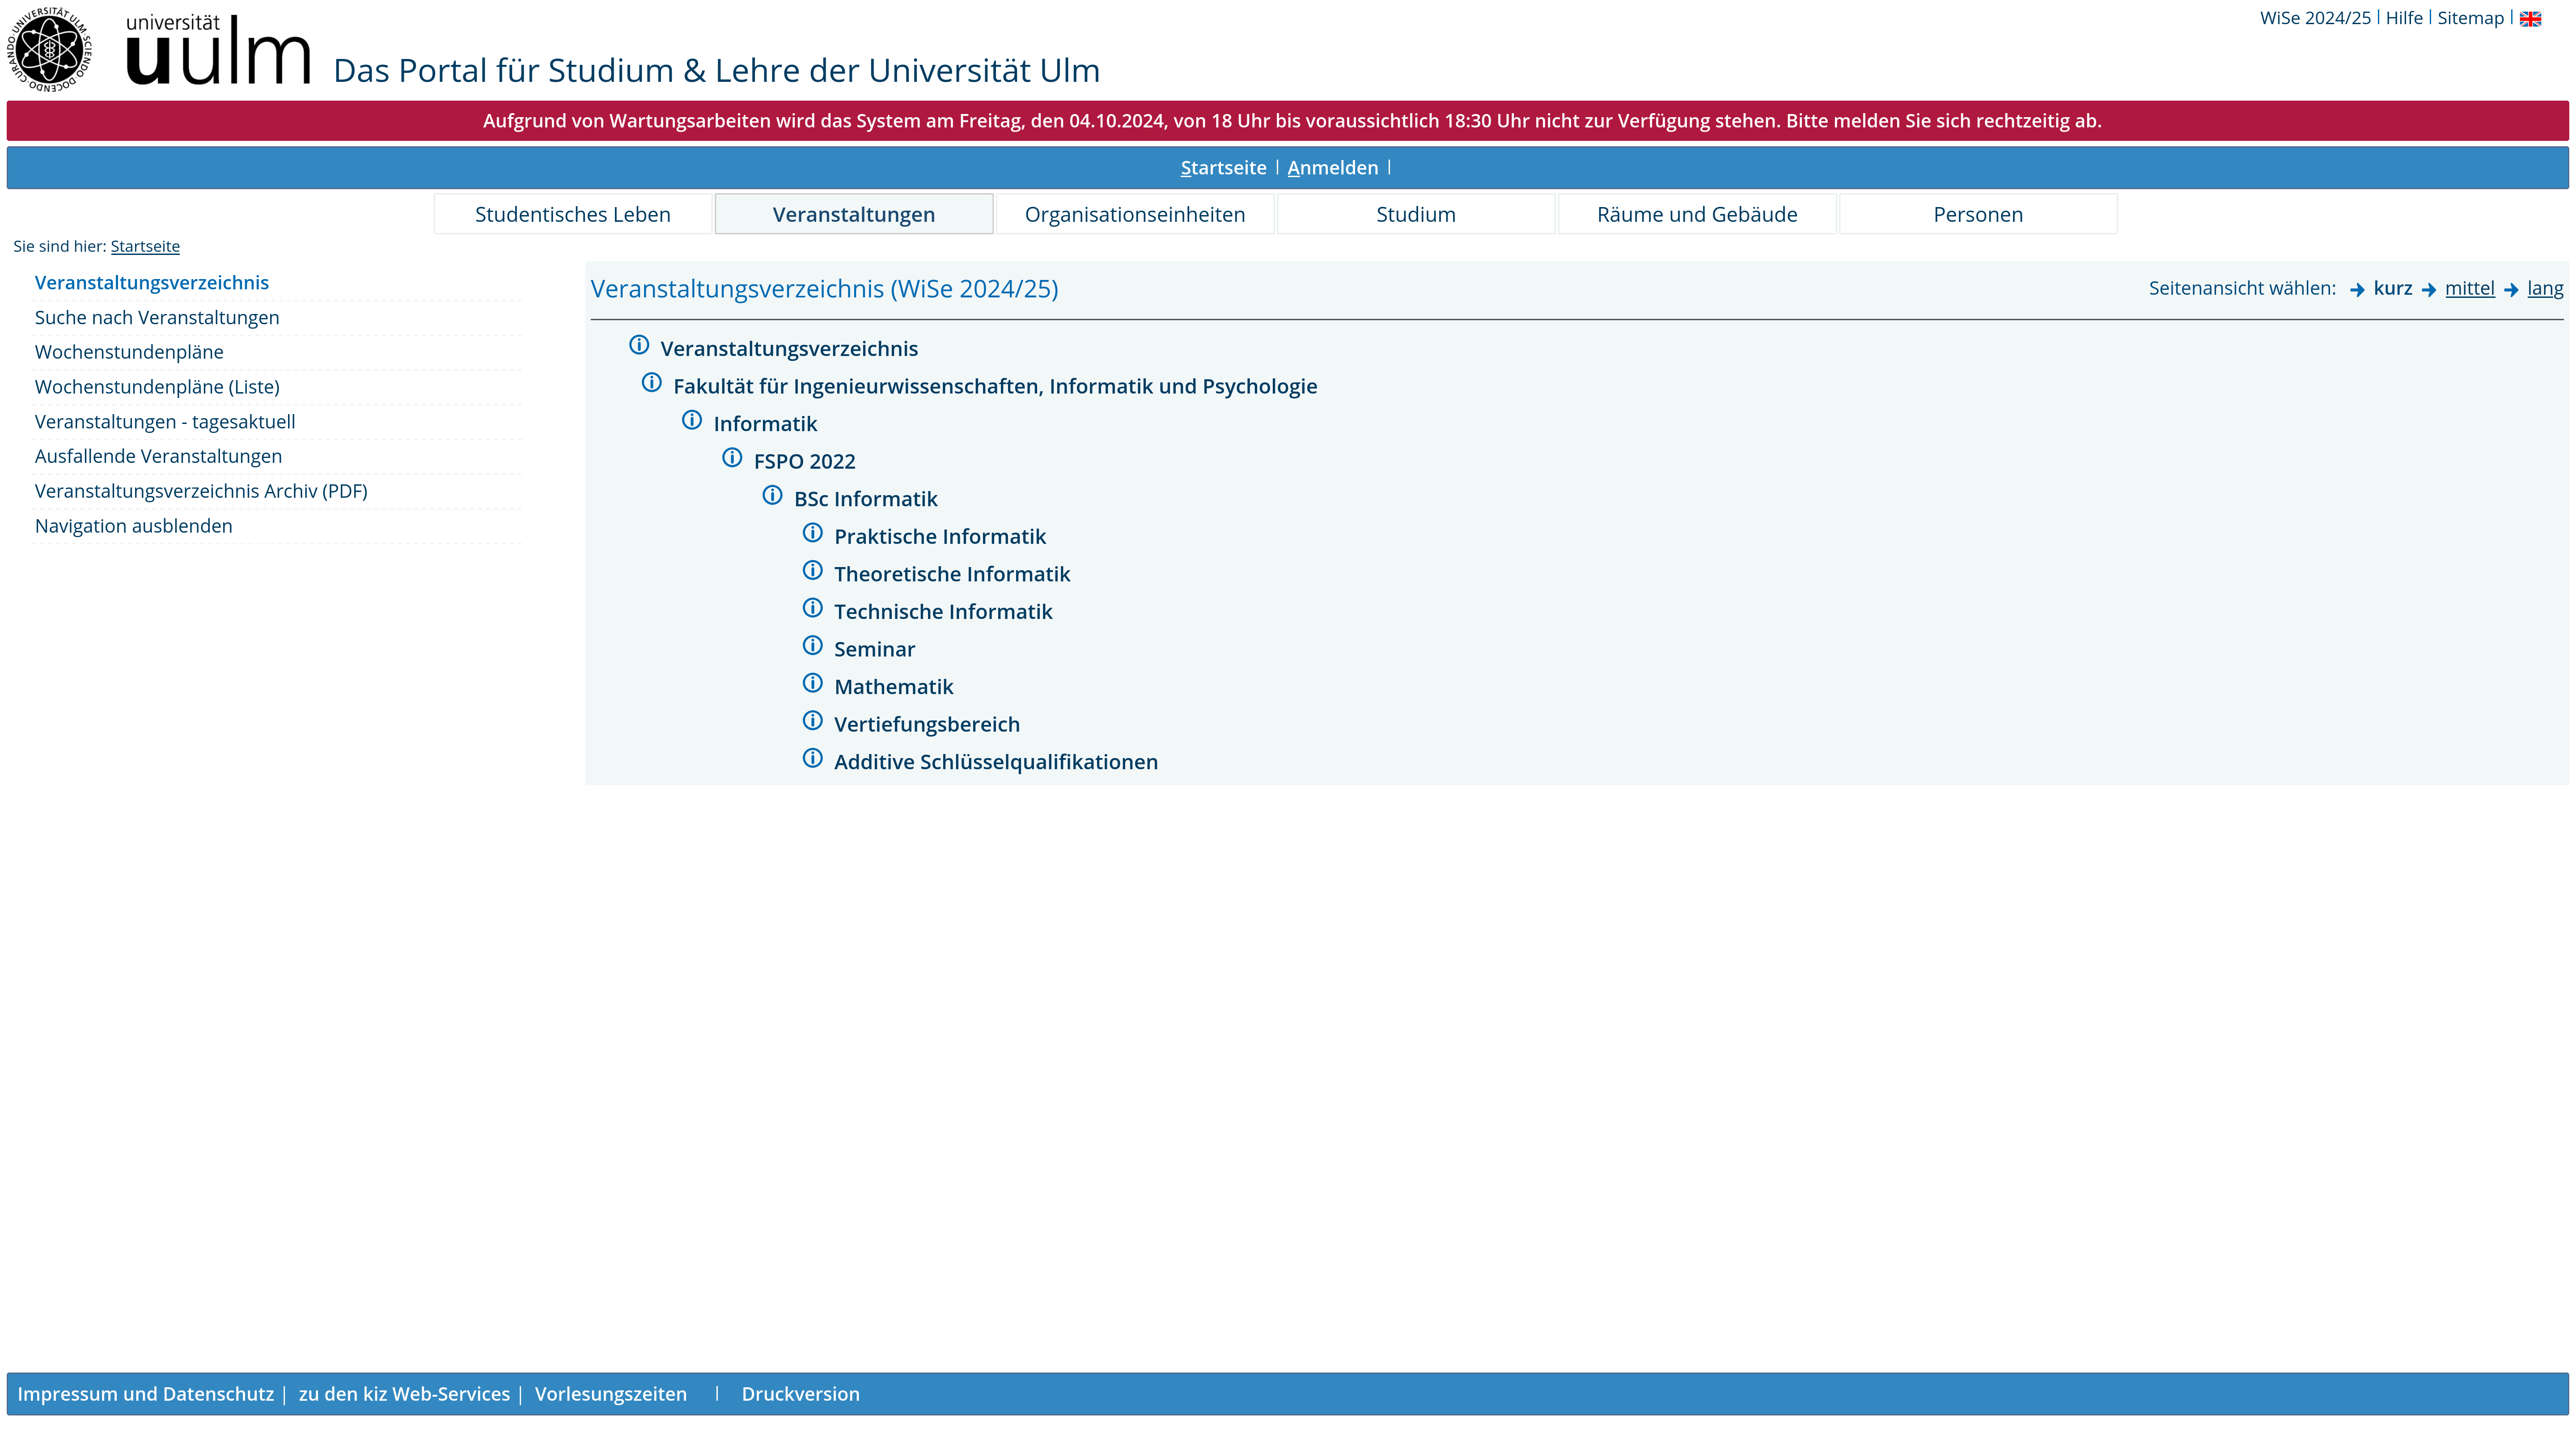
\includegraphics[clip, trim={0 10cm 0 0}, width=\linewidth]{assets/lsf-2.png}
\end{frame}

\begin{frame}{\insertsubsection \space|\space\underline{\href{https://campusonline.uni-ulm.de}{campusonline.uni-ulm.de}}}
    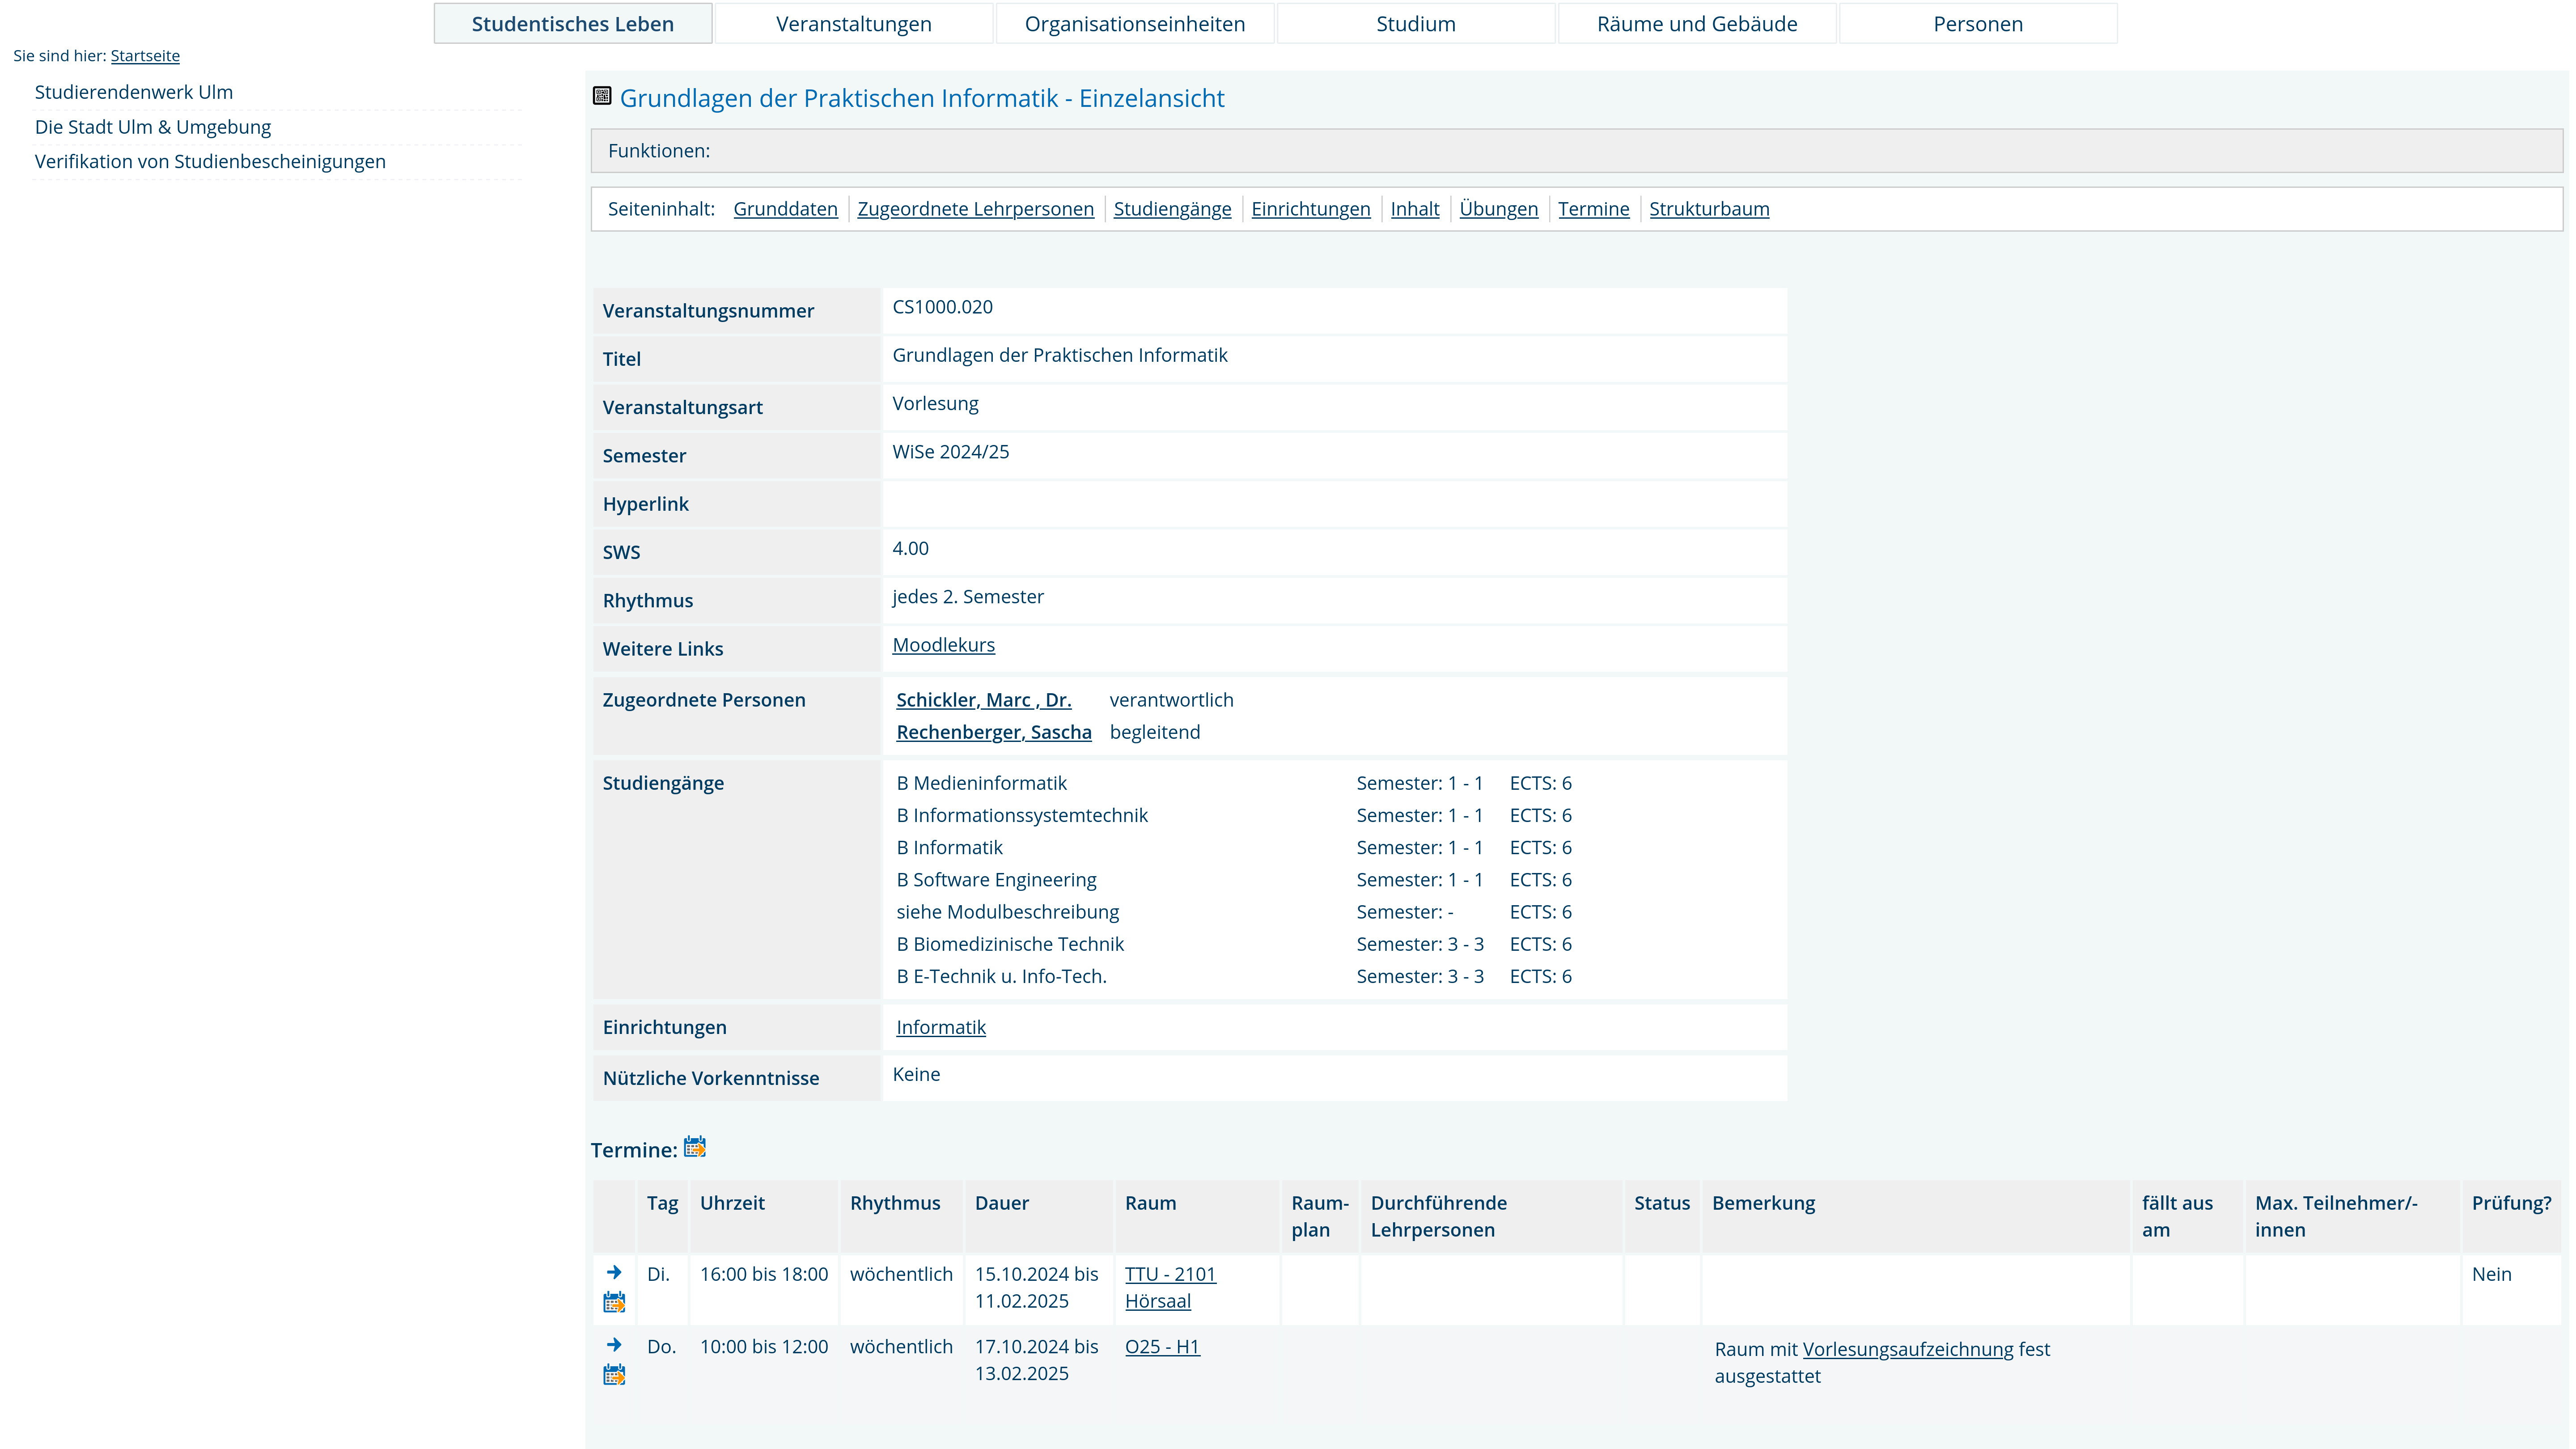
\includegraphics[clip, trim={0 10cm 0 5.5cm}, width=\linewidth]{assets/lsf-3.png}
\end{frame}

\begin{frame}{Prüfungsanmeldung \space|\space\underline{\href{https://campusonline.uni-ulm.de}{campusonline.uni-ulm.de}}}
    \begin{annotatedFigure}
        {\includegraphics[clip, trim={0 0 0 0}, width=\linewidth]{assets/exam.png}}
        \annotatedFigureBox{0.12,0.8287}{0.231,0.8812}{A}{0.12,0.8287}%bl
        \annotatedFigureBox{-0.004,0.7676}{0.091,0.7978}{B}{-0.004,0.7676}%bl
        \annotatedFigureBox{0.218,0.6645}{0.342,0.7071}{C}{0.218,0.6645}%bl
    \end{annotatedFigure}
\end{frame}

\subsection{Moodle}
\begin{frame}{\insertsubsection \space|\space\underline{\href{https://moodle.uni-ulm.de}{moodle.uni-ulm.de}}}
    \begin{itemize}
        \item Alle wichtigen Kursinformationen 
        \item Übungsblätter, Abgaben, Forum, Neuigkeiten
        \item Einschreiben in Kurse ist nicht verbindlich (Prüfungsanmeldung \underline{nur} über LSF)
    \end{itemize}
\end{frame}

\begin{frame}{\insertsubsection \space|\space\underline{\href{https://moodle.uni-ulm.de}{moodle.uni-ulm.de}}}
    \includegraphics[width=\linewidth]{assets/moodle-overview.png}
\end{frame}

\begin{frame}{\insertsubsection \space|\space\underline{\href{https://moodle.uni-ulm.de}{moodle.uni-ulm.de}}}
    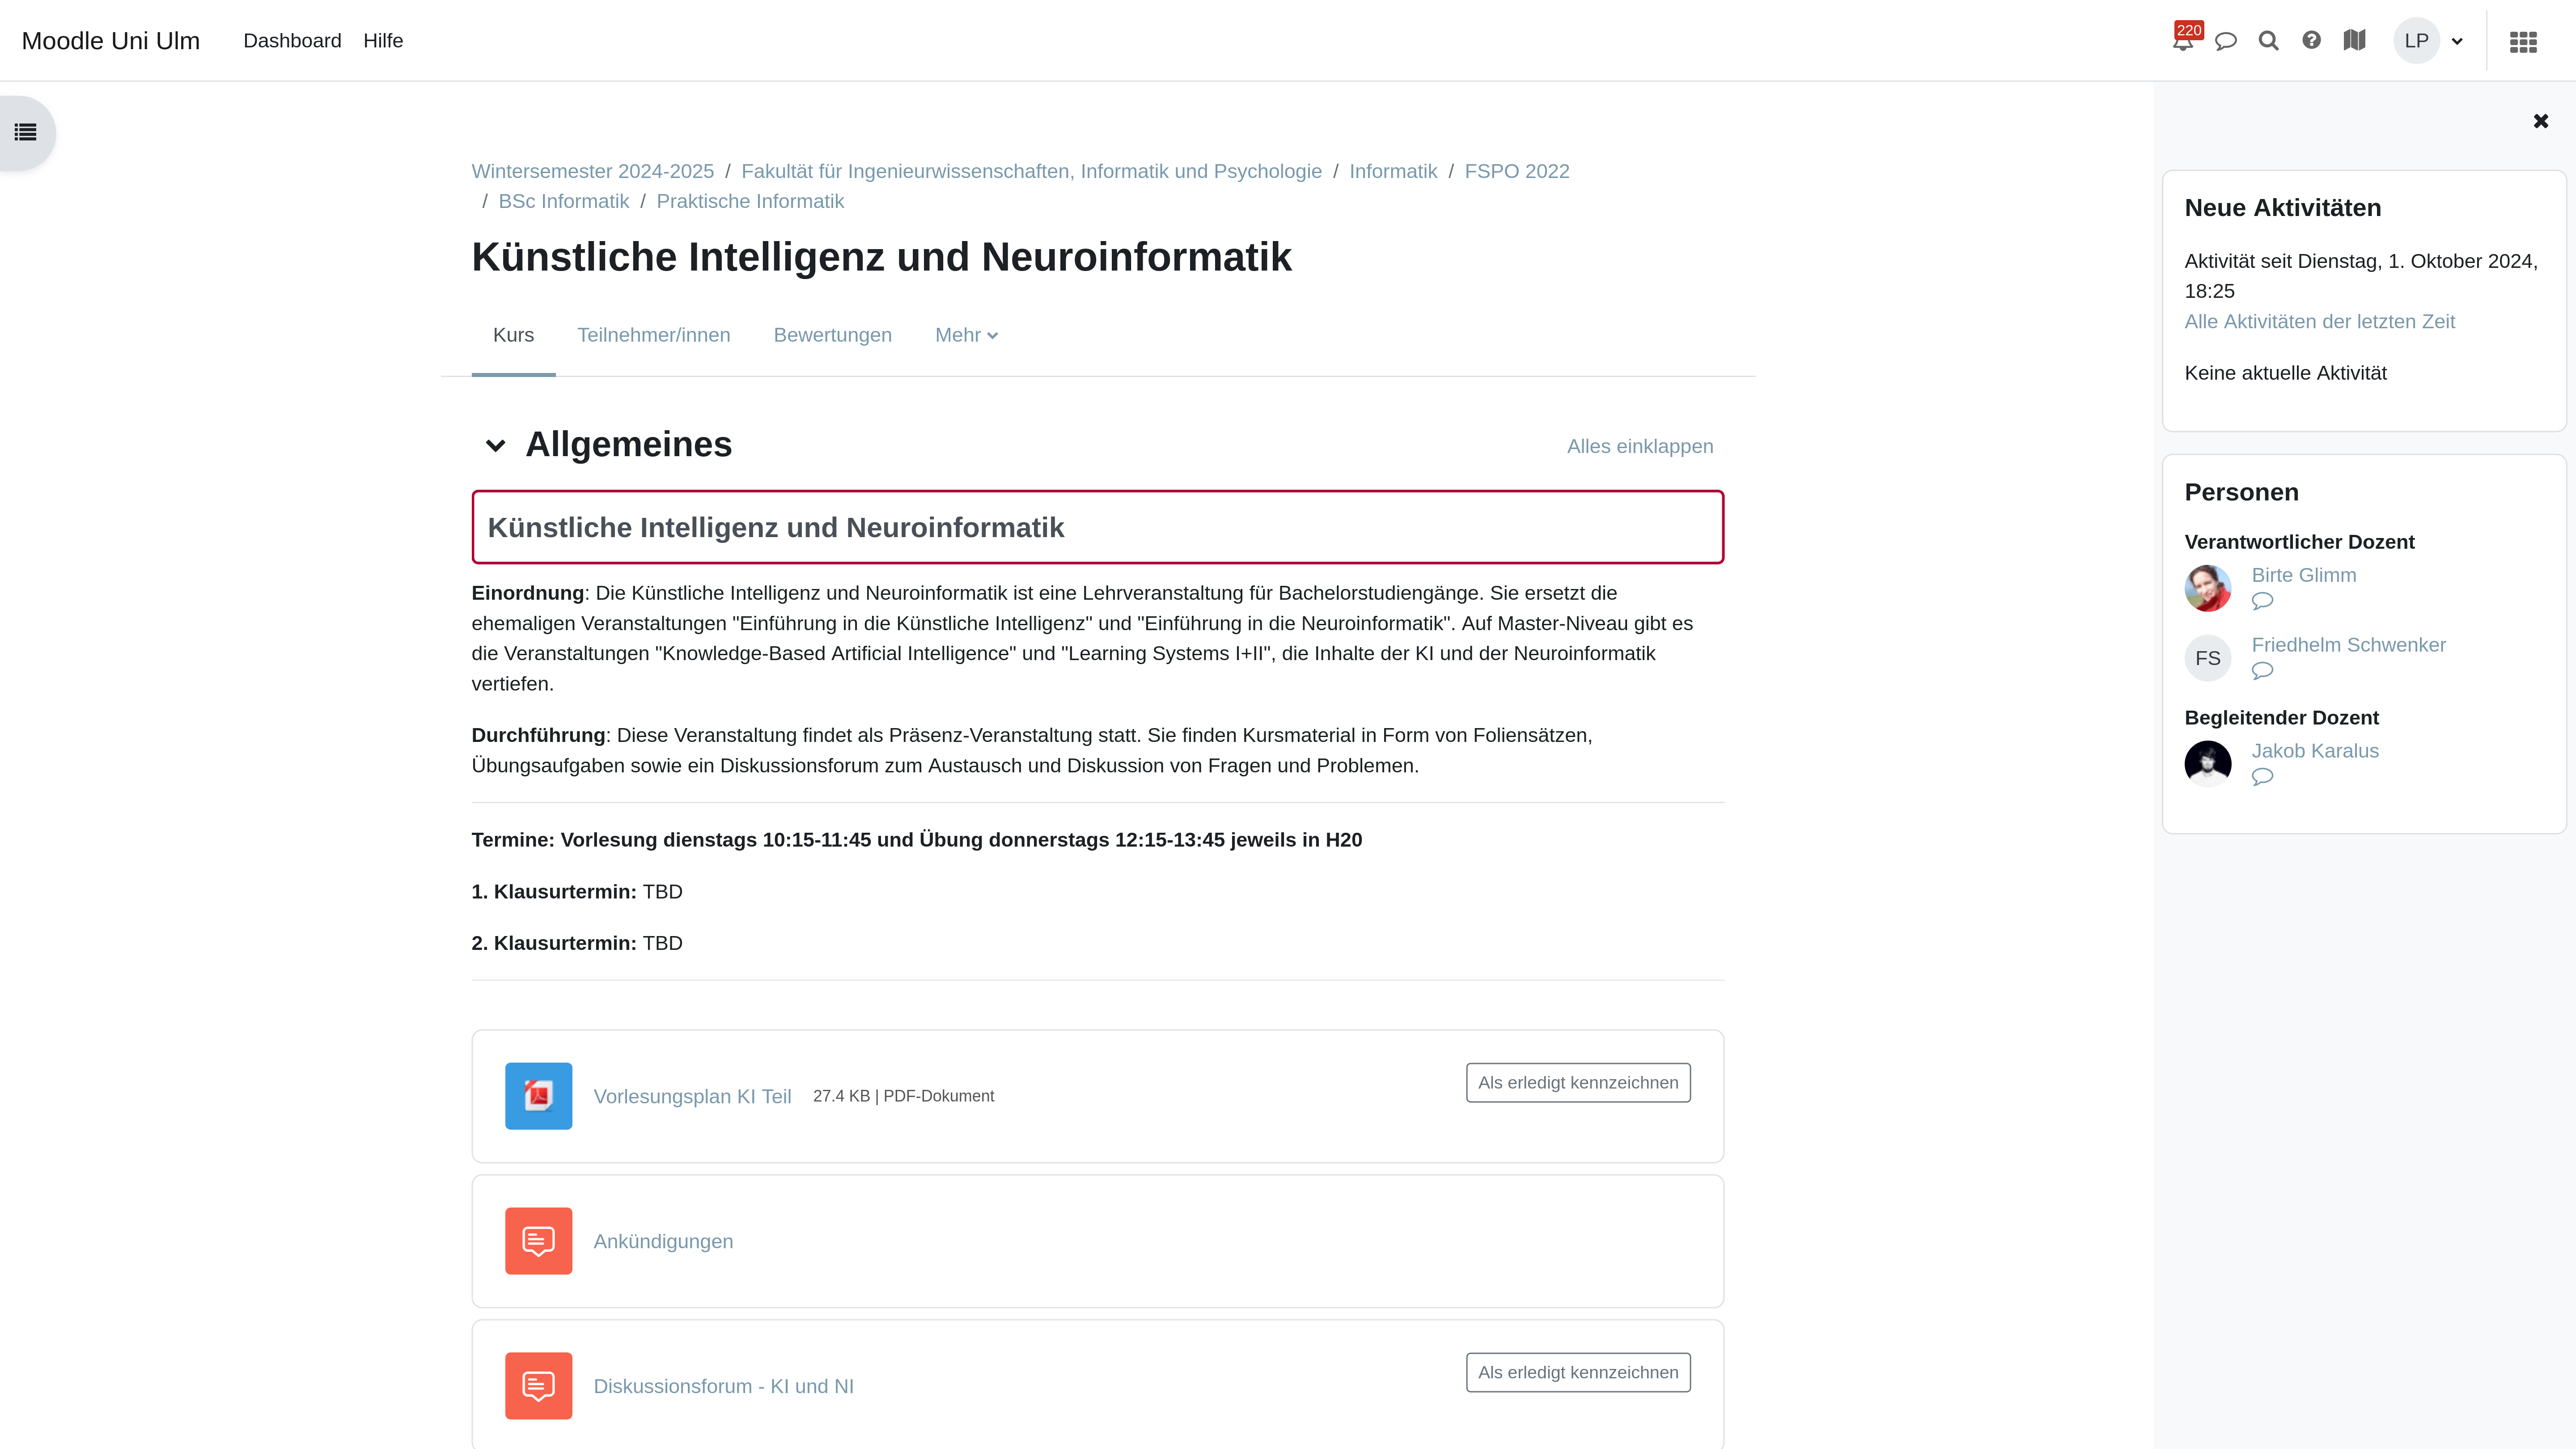
\includegraphics[width=\linewidth]{assets/moodle-course.png}
\end{frame}


\subsection{kiz Web-Services}
\begin{frame}{\insertsubsection \space|\space\underline{\href{https://portal.uni-ulm.de}{portal.uni-ulm.de}}}
    \begin{fancycolumns}[widths={60}]
        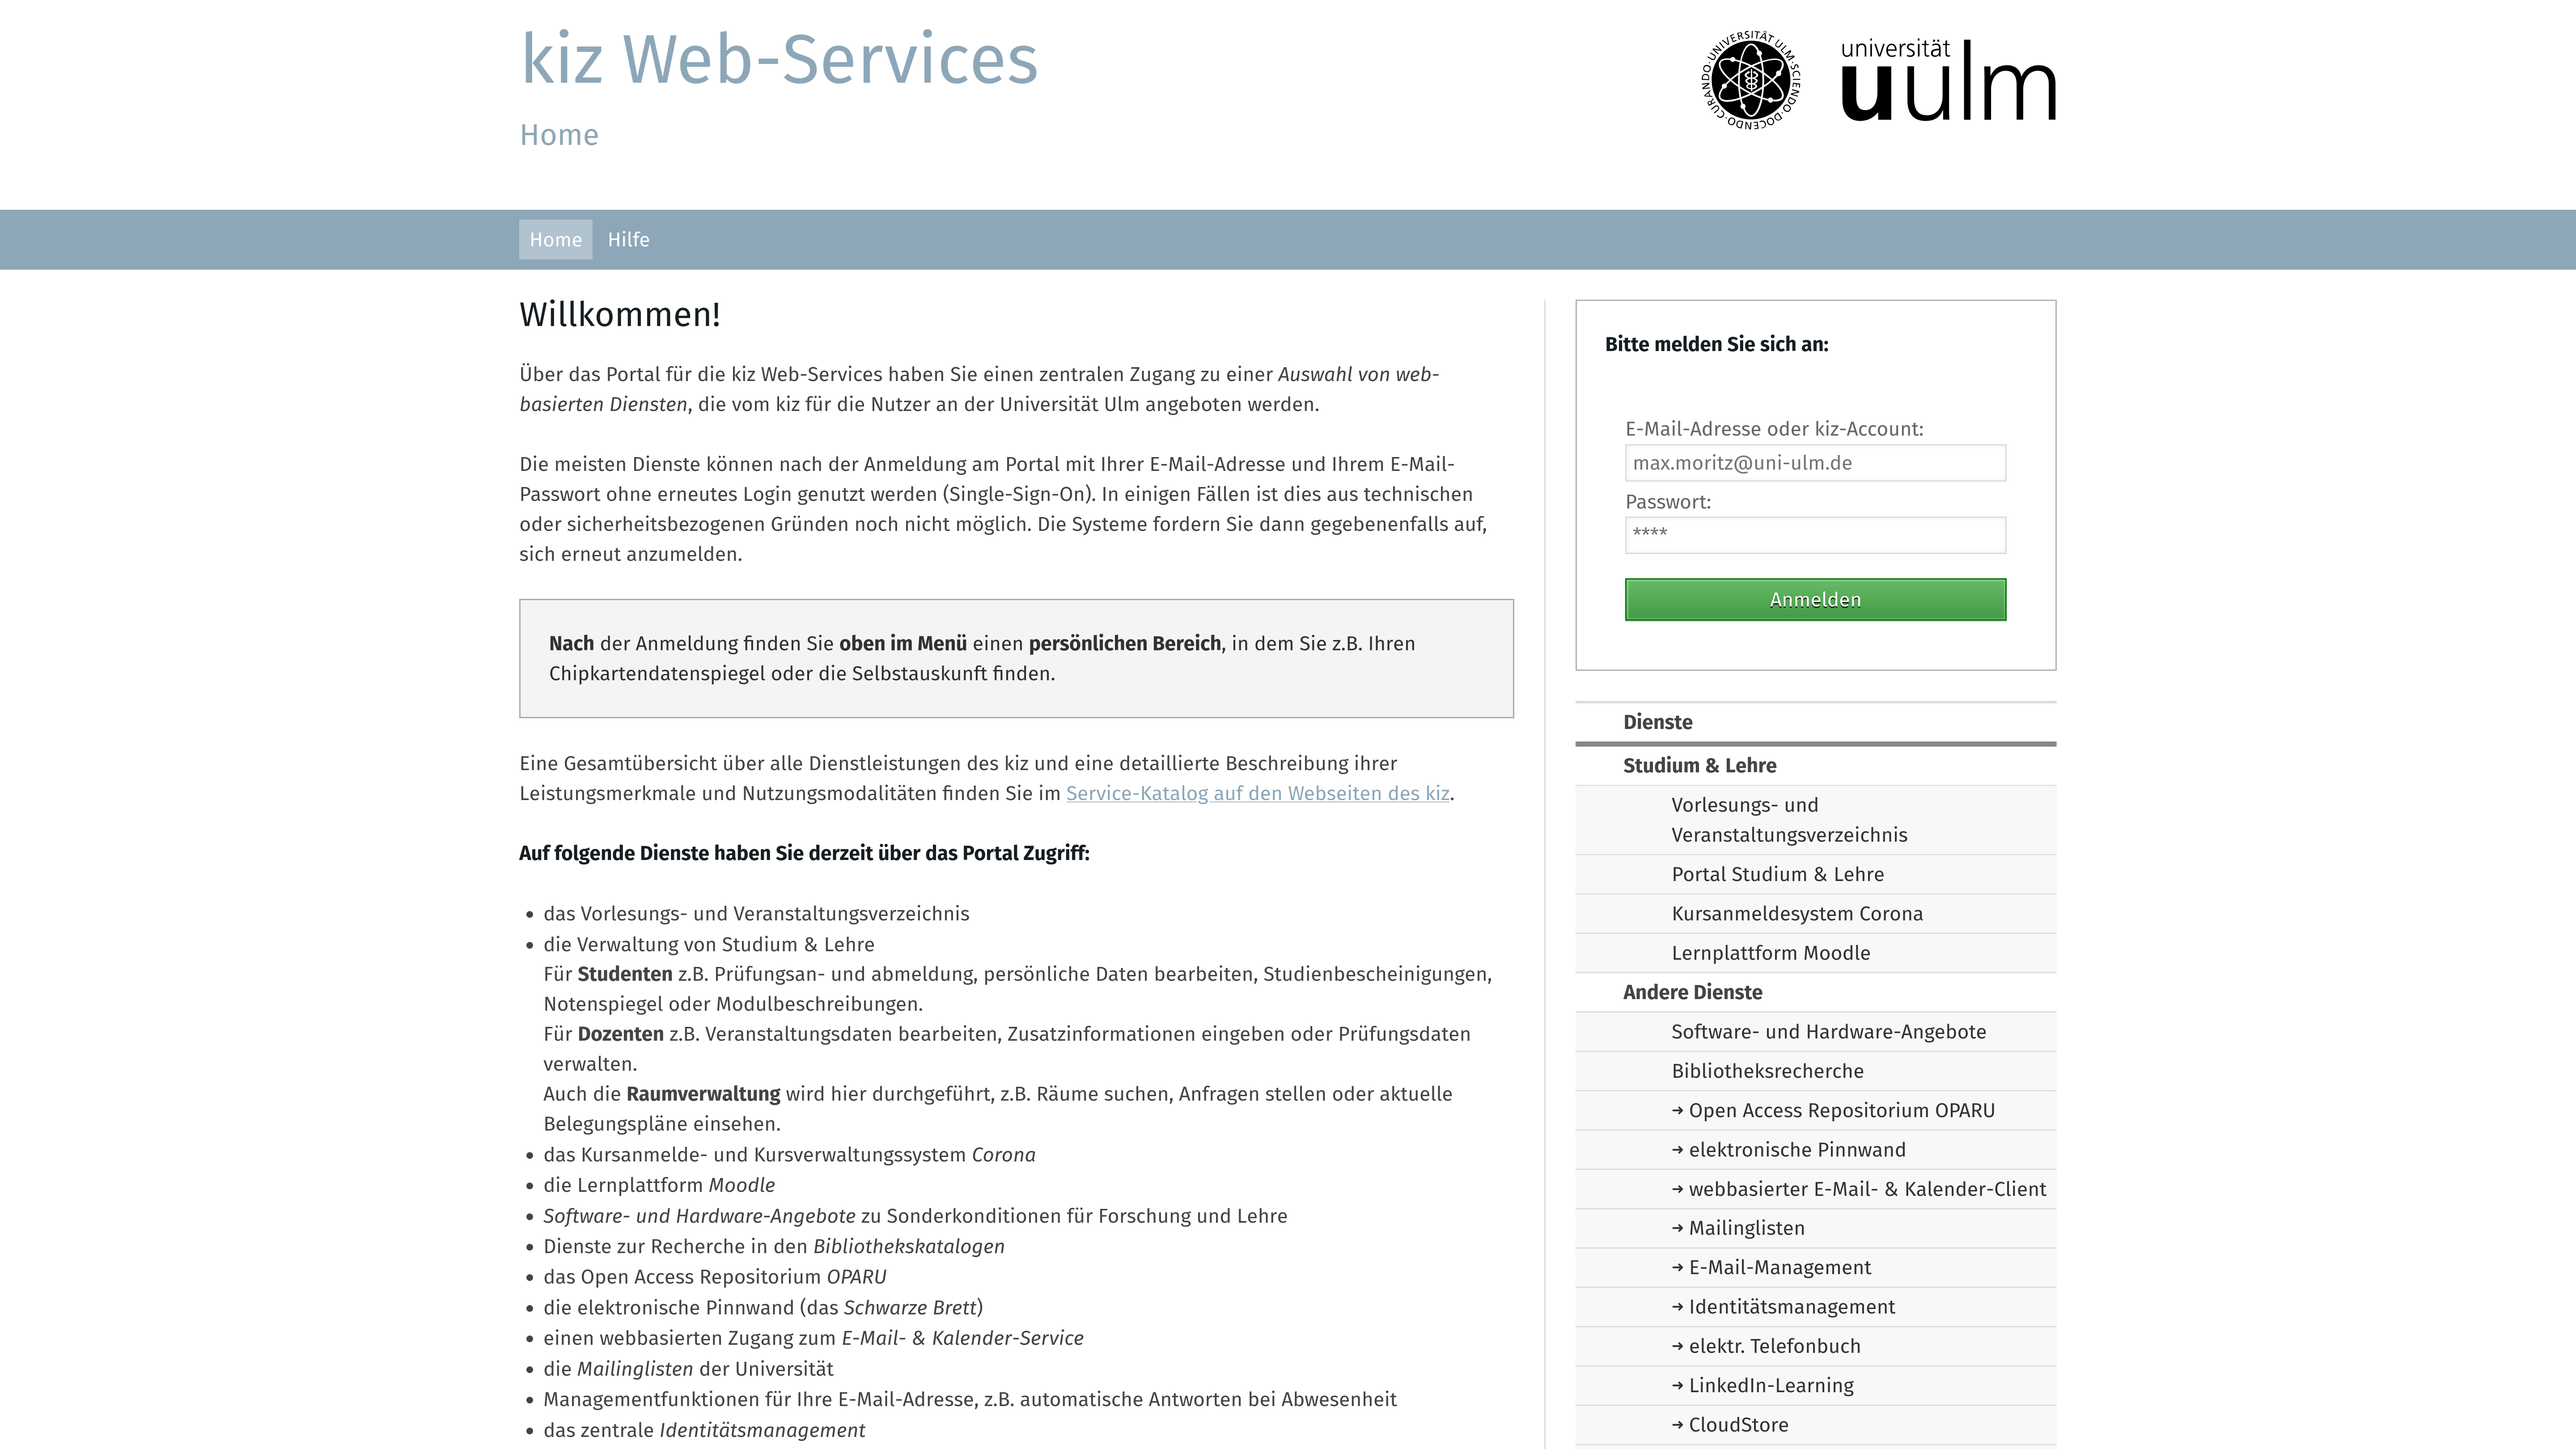
\includegraphics[clip, trim={30cm 0 30cm 0}, width=\linewidth]{assets/kiz.png}
        \nextcolumn
        \begin{itemize}
            \item Zugang zu allen Services
            \item Moodle, LSF, IDM, etc
            \item Einfache Anmeldung 
        \end{itemize}
    \end{fancycolumns}
\end{frame}

\subsection{Uni E-Mail}
\begin{frame}{\insertsubsection}
    \begin{fancycolumns}[T, widths={30}]
        \fancyqr[height=\linewidth]{https://www.uni-ulm.de/einrichtungen/kiz/service-katalog/e-mail-kalender-zusammenarbeit/e-mail/e-mail-programme-konfigurieren/}
        \begin{center}
            \textbf{Tutorial}: E-Mail-Programm konfigurieren
        \end{center}    
        \nextcolumn
        \begin{itemize}
            \item Format: \lstinline|vorname.nachname@uni-ulm.de|
            \item Wichtige Informationen und Benachrichtigungen von Moodle, LFS, etc.
            \item Über \underline{\href{https://sogo.uni-ulm.de}{sogo.uni-ulm.de}} lesen
            \item Empfehlung: \underline{\href{https://www.uni-ulm.de/einrichtungen/kiz/service-katalog/e-mail-kalender-zusammenarbeit/e-mail/e-mail-programme-konfigurieren/}{Uni Mail zur Mailapp hinzufügen}}
        \end{itemize}
    \end{fancycolumns}
\end{frame}


\section{Prüfungsordnungen}
\subsection{Was diese?}
\subsection{Welche Module im ersten Semester}
\subsection{Was ist ein Modul}
\subsection{Was ist eine Prüfung}
\subsection{Wie viele Versuche}
\subsection{Wann/wie an/abmelden}
\subsection{Orientierungsprüfungen}
\subsection{Bachelor Arbeit}
\subsection{Endnote}

\section{Leben an der Uni}
\subsection{Wie lernen?}
\subsection{Wo lernen?}
\subsection{Wo finde ich Räume?}
\subsection{Wo Altklausuren?}
\subsection{Ansprechpartner}
\subsection{Seite von der Fachschaft}


\section{Freizeit}
\subsection{Studibars}
\subsection{Hochschulsport}
\subsection{Referate}
\subsection{Ehrenamte}



\section{Schlussworte}
\begin{frame}{Ende}
\begin{center}
    Fragen - Feedback
\end{center}
\end{frame}


\end{document}